%!TEX program = xelatex
\documentclass[a4paper,14pt]{extarticle}

% === Кодировка и язык ===
\usepackage{fontspec}
\setmainfont{Liberation Serif}
\setsansfont{Liberation Sans}
\setmonofont{Liberation Mono}

\usepackage{polyglossia}
\setdefaultlanguage{russian}
\setotherlanguage{english}

% === Геометрия страницы ===
\usepackage{geometry}
\geometry{
  a4paper,
  left=30mm, right=15mm,
  top=20mm, bottom=20mm
}

% === Межстрочный интервал ===
\usepackage{setspace}
\onehalfspacing

% === Оглавление и заголовки ===
\usepackage{titlesec}
\titleformat{\section}{\normalfont\large\bfseries}{\thesection.}{0.5em}{}
\titleformat{\subsection}{\normalfont\normalsize\bfseries}{\thesubsection.}{0.5em}{}

% === Колонтитулы ===
\usepackage{fancyhdr}
\setlength{\headheight}{17pt}
\pagestyle{fancy}
\fancyhf{}
\fancyhead[R]{\thepage}
\renewcommand{\headrulewidth}{0pt}

% === Работа с рисунками, таблицами, листингами ===
\usepackage{graphicx}
\usepackage{caption}
\usepackage{listings}
\usepackage{xcolor}
\usepackage{tabularx}
\usepackage{booktabs}
\usepackage{array}
\usepackage{longtable}
\usepackage{float}

% === Листинги кода ===
\lstdefinestyle{Cstyle}{
  language=C,
  basicstyle=\small\ttfamily,
  keywordstyle=\bfseries\color{black},
  commentstyle=\itshape\color{gray},
  stringstyle=\color{black},
  numbers=left,
  numberstyle=\tiny,
  stepnumber=1,
  numbersep=6pt,
  breaklines=true,
  frame=single,
  tabsize=2,
  showstringspaces=false,
  extendedchars=true,
  inputencoding=utf8
}

\lstdefinestyle{ASMstyle}{
  basicstyle=\small\ttfamily,
  numbers=none,
  breaklines=true,
  frame=single,
  tabsize=8,
  showstringspaces=false
}

\lstdefinestyle{PLIstyle}{
  basicstyle=\small\ttfamily,
  numbers=none,
  breaklines=true,
  frame=single,
  showstringspaces=false
}

% === Гиперссылки ===
\usepackage[hidelinks]{hyperref}

% === Прочее ===
\usepackage{enumitem}
\usepackage{amsmath}
\usepackage{indentfirst}
\setlength{\parindent}{1.25cm}

% === Подписи к рисункам ===
\captionsetup[figure]{name=Рис.,labelsep=period}
\captionsetup[table]{name=Таблица,labelsep=period}

\begin{document}

% ============================================================
% ТИТУЛЬНЫЙ ЛИСТ
% ============================================================
\thispagestyle{empty}
\begin{center}
  \textbf{Санкт-Петербургский политехнический университет}\\
  \textbf{Институт компьютерных наук и технологий}\\
  \textbf{Высшая школа программной инженерии}\\[3cm]

  {\Large\textbf{К У Р С О В А Я \quad Р А Б О Т А}}\\[1cm]
  {\large Разработка учебной системы программирования}\\[0.5cm]
  {\large Компилятор с ЯВУ}\\[2cm]

  Дисциплина: «Системы программирования»\\[1cm]
  Вариант~№~11\\[2cm]
\end{center}

\begin{flushright}
  \begin{tabular}{ll}
    Исполнители: & Студенты группы~5140904/50102\\
                 & Сырбу~Г.~В.\\
                 & Федерова~С.~К.\\[0.5cm]
    Руководитель: & Расторгуев~В.~Я.\\
  \end{tabular}
\end{flushright}

\vfill
\begin{center}
  Санкт-Петербург\\
  2026
\end{center}

\newpage

% ============================================================
% СОДЕРЖАНИЕ
% ============================================================
\tableofcontents
\newpage

% ============================================================
% РАЗДЕЛ 1. ЗАДАНИЕ НА КУРСОВУЮ РАБОТУ
% ============================================================
\section{Задание на курсовую работу}

Задание на курсовую работу дано в следующей общей формулировке:

\begin{quote}
«Необходимо выполнить доработку элементов макета учебной системы
программирования до уровня, позволяющего обрабатывать «новые» для макета
конструкции языка высокого уровня, примененные в соответствующем варианте».
\end{quote}

Общая формулировка персонализирована в варианте~№~11, приведённом на рис.~\ref{fig:variant}.

\begin{figure}[H]
\centering
\begin{lstlisting}[style=PLIstyle]
EX11: PROC OPTIONS ( MAIN );
DCL A BIN FIXED INIT ( 3 );
DCL B DEC FIXED INIT ( 3 );
DCL C BIN FIXED;
C = A = ( B * 5 );
END EX11;
\end{lstlisting}
\caption{Персональный вариант~№~11}
\label{fig:variant}
\end{figure}

По договорённости с преподавателем в персональный вариант были внесены
изменения, касающиеся использования скобок в арифметических выражениях:
вложенное выражение со скобками было разделено на два последовательных
оператора присваивания. В результате была сформулирована следующая входная
программа (рис.~\ref{fig:variant_mod}):

\begin{figure}[H]
\centering
\begin{lstlisting}[style=PLIstyle]
EX11: PROC OPTIONS ( MAIN );
DCL A BIN FIXED INIT ( 3 );
DCL B DEC FIXED INIT ( 3 );
DCL C BIN FIXED;
C = B * 5;
C = A = C;
END EX11;
\end{lstlisting}
\caption{Модифицированный персональный вариант~№~11 (согласованный с преподавателем)}
\label{fig:variant_mod}
\end{figure}

Схема функционирования макета учебной системы программирования, являющегося
согласно заданию на КР одним из элементов исходных данных, приведена на рис.~\ref{fig:arch}.

\begin{figure}[H]
\centering
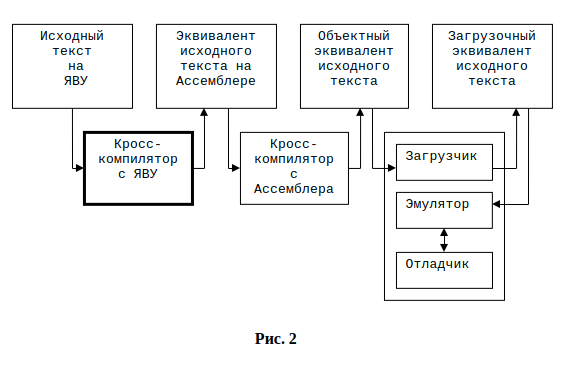
\includegraphics[width=\textwidth]{../источники/image.png}
\caption{Схема функционирования учебной системы программирования}
\label{fig:arch}
\end{figure}

Дополнительные требования к КР предполагают, что данная система программирования
работает на технологической ЭВМ (IBM PC) и является по существу кросс-системой для
объектной ЭВМ (IBM~370). В этой системе:
\begin{itemize}
  \item в качестве языка высокого уровня (ЯВУ) выбран язык, образованный из
        подмножества языковых конструкций PL/1; исходная программа готовится в виде
        текстового файла с расширением \texttt{*.pli};
  \item язык Ассемблера сформирован из языковых конструкций Ассемблера IBM~370;
        ассемблерный эквивалент исходной программы формируется в виде текстового
        файла с расширением \texttt{*.ass};
  \item объектный эквивалент исходной программы готовится в формате объектных файлов
        ОС IBM~370 и хранится в виде двоичного файла с расширением \texttt{*.tex};
  \item загрузочный эквивалент исходной программы представляет собой машинный код
        IBM~370, запоминаемый в области ОЗУ технологической ЭВМ, являющейся зоной
        загрузки для эмулятора объектной ЭВМ.
\end{itemize}

В данном отчёте документируются результаты модификации макетного компилятора с~ЯВУ
под персональный вариант~№~11.

\subsection*{Контрольный (демонстрационный) пример}

Контрольным примером, на который изначально настроен макет компилятора,
является программа \texttt{examppl.pli} (рис.~\ref{fig:demo}).

\begin{figure}[H]
\centering
\begin{lstlisting}[style=PLIstyle]
EXAMP: PROC OPTIONS ( MAIN );
DCL A BIN FIXED ( 31 ) INIT ( 11B  );
DCL B BIN FIXED ( 31 ) INIT ( 100B );
DCL C BIN FIXED ( 31 ) INIT ( 101B );
DCL D BIN FIXED ( 31 );
D = A + B - C;
END EXAMP;
\end{lstlisting}
\caption{Демонстрационный пример (\texttt{examppl.pli})}
\label{fig:demo}
\end{figure}

\subsection*{Отличия персонального варианта от демонстрационного примера}

Модифицированный персональный вариант~№~11 (рис.~\ref{fig:variant_mod})
приведён ниже:

\begin{lstlisting}[style=PLIstyle]
EX11: PROC OPTIONS ( MAIN );
DCL A BIN FIXED INIT ( 3 );
DCL B DEC FIXED INIT ( 3 );
DCL C BIN FIXED;
C = B * 5;
C = A = C;
END EX11;
\end{lstlisting}

При визуальном сравнении модифицированного персонального варианта~№~11
и демонстрационного примера (рис.~\ref{fig:demo}) выявлены следующие отличия:

\begin{enumerate}
  \item Переменные в персональном варианте объявляются без указания
        разрядности (без параметра в скобках), а инициализация задаётся
        десятичным целочисленным литералом (например, \texttt{3}) вместо
        двоичного (\texttt{11B}).

  \item В персональном варианте введена переменная \texttt{B} типа
        \texttt{DEC FIXED} (упакованный десятичный формат), тогда как в
        демонстрационном примере все переменные имеют тип \texttt{BIN FIXED}
        (двоичный формат с фиксированной точкой).

  \item В операторе \texttt{C = B * 5;} применяется операция умножения «\texttt{*}»
        упакованного десятичного операнда на десятичный целочисленный литерал,
        отсутствующая в демонстрационном примере.

  \item В операторе \texttt{C = A = C;} применяется знак логической операции
        «\texttt{=}» (сравнение) в правой части оператора присваивания,
        формирующий булево (логическое) значение — конструкция, отсутствующая
        в демонстрационном примере.
\end{enumerate}

% ============================================================
% РАЗДЕЛ 2. ПОСТАНОВКА ЗАДАЧИ
% ============================================================
\section{Постановка задачи модификации макета в части компилятора с ЯВУ}

Схема функционирования модифицированного макетного компилятора с~ЯВУ должна
соответствовать рис.~\ref{fig:compil_scheme}.

\begin{figure}[H]
\centering
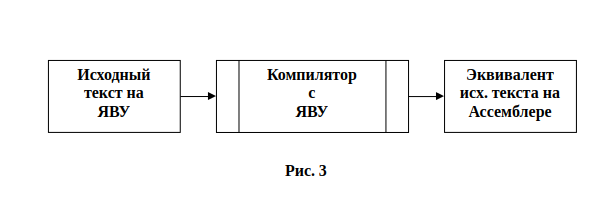
\includegraphics[width=\textwidth]{../источники/image2.png}
\caption{Схема функционирования модифицированного макетного компилятора с~ЯВУ}
\label{fig:compil_scheme}
\end{figure}

Функционал модифицированного макетного компилятора должен обеспечить компиляцию
исходного текста на ЯВУ (рис.~\ref{fig:variant_mod}) в эквивалент исходного текста на
Ассемблере, представленный на рис.~\ref{fig:etalon}.

\begin{figure}[H]
\centering
\begin{lstlisting}[style=ASMstyle]
  Метка       КОП       Операнды              Пояснения
EX11     START  0            Init rel addr=0
         BALR   @RBASE,0     Set @RBASE=cur PC
         USING  *,@RBASE     Use @RBASE for addr
         ZAP    @BUF(8),B(3) Copy pdec B->BUF
         MP     @BUF(8),@FIVE(1) Mul BUF by 5->BUF
         CVB    @R1,@BUF     pdec BUF ->int @R1
         STH    @R1,C        Store int ->C
         LH     @R2,A        Load A ->@R2
         CH     @R2,C        Compare @R2 with C
         BC     8,@TRUE      Branch if equal
         LA     @R3,0        Set @R3=0 (F)
         B      @SAVE        Jump to save
@TRUE    LA     @R3,1        Set @R3=1 (T)
@SAVE    STH    @R3,C        Store bool ->C
         BCR    15,@RVIX     Return to caller
A        DC     H'3'         Store halfword init
B        DC     PL3'3'       Store pdec init
C        DS     H            Reserve halfword
@FIVE    DC     PL1'5'       Store packed const
         DS     0F           Align next item
@BUF     DC     PL8'0'       Clear packed BUF
@RBASE   EQU    5            Set @RBASE=5
@R1      EQU    6            Set @R1=6
@R2      EQU    2            Set @R2=2
@R3      EQU    3            Set @R3=3
@RVIX    EQU    14           Set @RVIX=14
         END                 Program ends
\end{lstlisting}
\caption{Эталон ассемблерного эквивалента персонального варианта~№~11}
\label{fig:etalon}
\end{figure}

% ============================================================
% РАЗДЕЛ 3. МОДИФИКАЦИЯ БД КОМПИЛЯТОРА
% ============================================================
\section{Модификация состава и структуры БД макета компилятора с ЯВУ}

\subsection{Модификация БД лексического анализатора}

БД лексического анализатора определяется путём выделения подмножества терминальных
символов-разделителей термов языка. Функция лексического анализа в макете реализована
в подпрограмме \texttt{compress\_ISXTXT()}.

Для персонального варианта~№~11 разделителями термов являются терминальные символы
из множества:
\[
  \{\,\texttt{":"}\,,\, \texttt{"("}\,,\, \texttt{")"}\,,\, \texttt{";"}\,,\,
     \texttt{"+"}\,,\, \texttt{"-"}\,,\, \texttt{"="}\,,\, \texttt{"\_"}\,,\,
     \texttt{"*"}\,\}
\]

Модификация лексических настроек демонстрационного примера состоит в добавлении
символа умножения «\texttt{*}» в перечень разделителей термов. Данный символ в
оригинальном макете не входил в число обрабатываемых разделителей. Поскольку авторы
макета разместили перечень символов-разделителей непосредственно в теле подпрограммы
\texttt{compress\_ISXTXT()}, модификация выполнена в теле этой подпрограммы:

\begin{lstlisting}[style=Cstyle,caption={Фрагмент \texttt{compress\_ISXTXT()} с добавленным символом «\texttt{*}»},label=lst:lex]
void compress_ISXTXT()
{
  /* ... */
  if (
    ( ISXTXT[I1][I2] == '+' ||
      ISXTXT[I1][I2] == '-' ||
      ISXTXT[I1][I2] == '=' ||
      ISXTXT[I1][I2] == '(' ||
      ISXTXT[I1][I2] == ')' ||
      ISXTXT[I1][I2] == '*'   /* <- добавлен разделитель '*' */
    )
    && PREDSYM == ' '
  )
  { I3--; goto L1; }

  if ( ISXTXT[I1][I2] == ' ' &&
     ( PREDSYM == '+' || PREDSYM == '-' ||
       PREDSYM == '=' || PREDSYM == '*'   /* <- добавлен '*' */
     )
  )
  { goto L2; }
  /* ... */
}
\end{lstlisting}

\subsection{Модификация БД синтаксического анализатора}

Высокоуровневое определение модифицированного синтаксиса для персонального
варианта~№~11 приведено ниже; модификации по сравнению с грамматикой
демонстрационного примера выделены курсивом:

\begin{enumerate}
  \item $\langle\text{PRO}\rangle ::= \langle\text{OPR}\rangle\langle\text{TEL}\rangle\langle\text{OEN}\rangle$
  \item $\langle\text{OPR}\rangle ::= \langle\text{IPR}\rangle\texttt{:PROC\_OPTIONS(MAIN);}$
  \item $\langle\text{IPR}\rangle ::= \langle\text{IDE}\rangle$
  \item $\langle\text{IDE}\rangle ::= \langle\text{BUK}\rangle \mid \langle\text{IDE}\rangle\langle\text{BUK}\rangle \mid \langle\text{IDE}\rangle\langle\text{CIF}\rangle$
  \item $\langle\text{BUK}\rangle ::= \texttt{A} \mid \texttt{B} \mid \texttt{C} \mid \texttt{D} \mid \texttt{E} \mid \texttt{M} \mid \texttt{P} \mid \texttt{X}$
  \item $\langle\text{CIF}\rangle ::= \texttt{0} \mid \texttt{1} \mid \texttt{2} \mid \texttt{3} \mid \texttt{4} \mid \texttt{5} \mid \texttt{6} \mid \texttt{7} \mid \texttt{8} \mid \texttt{9}$
  \item $\langle\text{TEL}\rangle ::= \langle\text{ODC}\rangle \mid \langle\text{TEL}\rangle\langle\text{ODC}\rangle \mid \langle\text{TEL}\rangle\langle\text{OPA}\rangle$
  \item $\langle\text{ODC}\rangle ::= \texttt{DCL\_}\langle\text{IPE}\rangle\texttt{\_BIN\_FIXED(}\langle\text{RZR}\rangle\texttt{);}$\\
        $\mid\; \texttt{DCL\_}\langle\text{IPE}\rangle\texttt{\_BIN\_FIXED(}\langle\text{RZR}\rangle\texttt{)INIT(}\langle\text{LIT}\rangle\texttt{);}$\\
        \textit{$\mid\; \texttt{DCL\_}\langle\text{IPE}\rangle\texttt{\_DEC\_FIXED(}\langle\text{RZR}\rangle\texttt{);}$}\\
        \textit{$\mid\; \texttt{DCL\_}\langle\text{IPE}\rangle\texttt{\_DEC\_FIXED(}\langle\text{RZR}\rangle\texttt{)INIT(}\langle\text{LIT}\rangle\texttt{);}$}\\
        \textit{$\mid\; \texttt{DCL\_}\langle\text{IPE}\rangle\texttt{\_BIN\_FIXED;}$}\\
        \textit{$\mid\; \texttt{DCL\_}\langle\text{IPE}\rangle\texttt{\_BIN\_FIXED\_INIT(}\langle\text{LID}\rangle\texttt{);}$}\\
        \textit{$\mid\; \texttt{DCL\_}\langle\text{IPE}\rangle\texttt{\_DEC\_FIXED;}$}\\
        \textit{$\mid\; \texttt{DCL\_}\langle\text{IPE}\rangle\texttt{\_DEC\_FIXED\_INIT(}\langle\text{LID}\rangle\texttt{);}$}
  \item $\langle\text{IPE}\rangle ::= \langle\text{IDE}\rangle$
  \item $\langle\text{RZR}\rangle ::= \langle\text{CIF}\rangle \mid \langle\text{RZR}\rangle\langle\text{CIF}\rangle$
  \item $\langle\text{LIT}\rangle ::= \langle\text{MAN}\rangle\texttt{B}$
  \item $\langle\text{MAN}\rangle ::= \texttt{1} \mid \langle\text{MAN}\rangle\texttt{0} \mid \langle\text{MAN}\rangle\texttt{1}$
  \item \textit{$\langle\text{LID}\rangle ::= \langle\text{CIF}\rangle \mid \langle\text{LID}\rangle\langle\text{CIF}\rangle$}
  \item $\langle\text{OPA}\rangle ::= \langle\text{IPE}\rangle\texttt{=}\langle\text{AVI}\rangle\texttt{;}$
  \item $\langle\text{AVI}\rangle ::= \langle\text{LIT}\rangle \mid $\textit{$\langle\text{LID}\rangle$}$\mid \langle\text{IPE}\rangle$\\
        $\mid\; \langle\text{AVI}\rangle\langle\text{ZNK}\rangle\langle\text{LIT}\rangle$
        \textit{$\mid\; \langle\text{AVI}\rangle\langle\text{ZNK}\rangle\langle\text{LID}\rangle$}
        $\mid\; \langle\text{AVI}\rangle\langle\text{ZNK}\rangle\langle\text{IPE}\rangle$\\
        \textit{$\mid\; \langle\text{AVI}\rangle\langle\text{ZNL}\rangle\langle\text{LIT}\rangle$}
        \textit{$\mid\; \langle\text{AVI}\rangle\langle\text{ZNL}\rangle\langle\text{LID}\rangle$}
        \textit{$\mid\; \langle\text{AVI}\rangle\langle\text{ZNL}\rangle\langle\text{IPE}\rangle$}
  \item $\langle\text{ZNK}\rangle ::= \texttt{+} \mid \texttt{-}$ \textit{$\mid\; \texttt{*}$}
  \item \textit{$\langle\text{ZNL}\rangle ::= \texttt{=}$}
  \item $\langle\text{OEN}\rangle ::= \texttt{END\_}\langle\text{IPR}\rangle$
\end{enumerate}

Пояснения к метасимволам:
\begin{itemize}
  \item \texttt{<} и \texttt{>} — ограничители нетерминального символа;
  \item \texttt{::=} — «равно по определению»;
  \item \texttt{|} — альтернативное определение («или»);
  \item \texttt{\_} — терминальный символ «пробел».
\end{itemize}

Перечень нетерминальных символов приведён в таблице~\ref{tab:nonterm}.

\begin{table}[H]
\centering
\caption{Нетерминальные символы грамматики}
\label{tab:nonterm}
\begin{tabularx}{\textwidth}{|l|X|}
  \hline
  \textbf{Нетерминал} & \textbf{Смысл} \\
  \hline
  \texttt{<PRO>} & программа \\
  \texttt{<OPR>} & оператор пролога программы \\
  \texttt{<IPR>} & имя программы \\
  \texttt{<IDE>} & идентификатор \\
  \texttt{<BUK>} & буква \\
  \texttt{<CIF>} & цифра \\
  \texttt{<TEL>} & тело программы \\
  \texttt{<ODC>} & оператор объявления переменных (DCL) \\
  \texttt{<IPE>} & имя переменной \\
  \texttt{<RZR>} & разрядность \\
  \texttt{<LIT>} & двоичный литерал \\
  \texttt{<MAN>} & мантисса литерала \\
  \texttt{<LID>} & десятичный целочисленный литерал \\
  \texttt{<OPA>} & оператор присваивания \\
  \texttt{<AVI>} & арифметическое выражение \\
  \texttt{<ZNK>} & знак арифметической операции \\
  \texttt{<ZNL>} & знак логической операции \\
  \texttt{<OEN>} & оператор эпилога программы (END) \\
  \hline
\end{tabularx}
\end{table}

По сравнению с грамматикой демонстрационного примера модифицированы правила:
\begin{itemize}
  \item \textbf{Правило~8 (\texttt{<ODC>}):} добавлены альтернативные
        правила для объявления переменных типа \texttt{DEC FIXED} — без
        инициализации и с инициализацией (с разрядностью и двоичным литералом
        для совместимости с демонстрационным примером); а также добавлены
        четыре новых альтернативы для объявления переменных без указания
        разрядности — \texttt{BIN FIXED} и \texttt{DEC FIXED}, без инициализации
        и с инициализацией десятичным целочисленным литералом \texttt{<LID>};
  \item \textbf{Правило~13 (\texttt{<LID>}):} введён новый нетерминал
        для десятичного целочисленного литерала (аналог \texttt{<LIT>} для
        десятичной записи), используемый при объявлении переменных без
        разрядности и в арифметических выражениях;
  \item \textbf{Правило~15 (\texttt{<AVI>}):} добавлена возможность применения
        нетерминала~\texttt{<LID>} (десятичного целочисленного литерала) как
        самостоятельного операнда выражения, а также добавлены альтернативы
        с участием знака логической операции \texttt{<ZNL>} для поддержки
        операции сравнения в правой части присваивания;
  \item \textbf{Правило~16 (\texttt{<ZNK>}):} знак «\texttt{=}» вынесен
        из множества арифметических операций в отдельный нетерминал;
        добавлен знак «\texttt{*}» (умножение);
  \item \textbf{Правило~17 (\texttt{<ZNL>}):} введён новый нетерминал
        для знака логической операции «\texttt{=}» (сравнение),
        отделённый от знаков арифметических операций; различение
        арифметического и логического знаков производится по контексту
        их использования в грамматике.
\end{itemize}

В состав нетерминальных символов после модификации добавлены два новых
нетерминала: \texttt{<LID>} (десятичный целочисленный литерал) и
\texttt{<ZNL>} (знак логической операции).

\subsubsection*{Модификация таблицы синтаксических правил \texttt{SINT[]}}

Таблица \texttt{SINT[]} реализует двунаправленный список с альтернативными
ветвлениями, в котором каждая запись описывает один шаг распознавания (форма
распознавания — от правой части к нетерминалу). В ходе модификации:

\begin{itemize}
  \item размер таблицы увеличен; добавлены записи, описывающие новые
        ветки грамматики: альтернативы объявлений \texttt{ODC} без разрядности
        с использованием нетерминала \texttt{<LID>}, ветка распознавания
        нетерминала \texttt{<ZNL>} для знака логической операции «\texttt{=}»,
        а также ветки для \texttt{<LID>} в качестве операнда выражения
        \texttt{<AVI>};
  \item в существующих записях изменены поля альтернативы \texttt{ALT}
        для обеспечения перехода к новым веткам грамматики.
\end{itemize}

\end{document}
